%%%%%%%%%%%%%%%%%%%%%%%%%%%%%%%%%%%%%%%%%%%%%%%%%%%%%%%%%%%%%%%%%%%%%%%%%%%%%%%%
%
% NOTE TO AIP TYPSETERS: TO CONVERT FROM TWO-COL TO PREPRINT, SWITCH
% COMMENTOUT COMMAND FROM A TO B IE. use
\newcommand{\commentoutA}[1]{} 
\newcommand{\commentoutB}[1]{#1}
% instead of the following
%\newcommand{\commentoutA}[1]{#1}
%\newcommand{\commentoutB}[1]{}
\renewcommand{\thefootnote}{\fnsymbol{footnote}}

\commentoutA{\documentclass[prl,aps,twocolumn,showpacs,twocolumngrid,superbib]{revtex4}}
\commentoutB{\documentclass[prb,aps,nobibnotes,showpacs,superbib,preprint]{revtex4}}

\usepackage{graphicx}
\usepackage{amsfonts}
\usepackage{amsmath}
\usepackage{bm}
\usepackage{alltt}
\usepackage{dcolumn} 
\usepackage{amsmath} 
\usepackage{graphicx}
\makeatletter 
\makeatother

\newcommand{\Kxc}{{\bf K}_{\mathrm{xc}}}
\newcommand{\Np}{N_{\mathrm{p}}} \newcommand{\Nbox}{N_{\mathrm{b}}}

\begin{document}
\title[Short Title]{ Linear Scaling Computation of the Fock Matrix. VI. \\ 
                     Data Parallel Computation of the Exchange-Correlation Matrix.\footnotemark[4] }

\author{Chee Kwan Gan\footnotemark[2]}
\author{Matt Challacombe\footnotemark[3]}
 
\affiliation{ Theoretical Division,\\ Group T-12, MS B268, Los Alamos
              National Laboratory,\\ Los Alamos, New Mexico 87545}


\date{Oct 31, 2002}

\begin{abstract}
Recently, early onset linear scaling computation of the
exchange-correlation matrix has been achieved using Hierarchical
Cubature [J. Chem. Phys. {\bf 113}, 10037 (2000)]. Hierarchical
Cubature differs from other methods in that the integration grid is
adaptive and purely Cartesian, which allows for a straightforward
domain decomposition in parallel computations; the volume enclosing
the entire grid may be simply divided into a number of non-overlapping
boxes. In our data parallel approach, each box requires only a fraction 
of the total density to perform the necessary numerical integrations
due to the finite extent of Gaussian-Orbital basis sets.  This inherent 
data locality may be exploited to reduce communications between processors 
as well as to avoid memory and copy overheads associated with data 
replication.  Although the Hierarchical Cubature grid is Cartesian, 
naive boxing leads to irregular work loads due to strong spatial variations 
of the grid and the electron density.  In this paper we
\commentoutA{describe {\bf Equal Time partitioning},}
\commentoutB{describe      Equal Time partitioning,}
which employs time measurement of the smallest sub-volumes
(corresponding to the primitive cubature rule) to load balance
grid-work for the next self-consistent-field iteration.  After start
up from a heuristic Center of Mass partitioning, Equal Time
partitioning exploits smooth variation of the density and grid between
iterations to achieve a good load balance. In particular, speedups for
Equal Time partitioning applied to taxol (62 heavy atoms) were found
to be 61 out of 64 processors, and 113 out of 128 processors for a 110
molecule water cluster at standard density.  For more coarse grained
calculations, superlinear speedups are obtained, resulting from
combination of a good load balance with a reduced computational
complexity due to data parallelism.

\smallskip
\noindent{\bf Keywords}: Density Functional Theory, linear scaling, numerical integration, Gaussian-Orbital, 
                         hierarchical methods, adaptive grid, load balance, parallel computation
\end{abstract}

\pacs{31.15.-p; 31.15.Ew; 02.60.Jh} 

%\keywords{Density Functional Theory, numerical integration, Gaussian-Orbital,linear scaling, 
%          hierarchical methods, adaptive grid, load balance, parallel computation}

\maketitle

\footnotetext[2]{\tt CKGan@LANL.Gov}
\footnotetext[3]{\tt MChalla@LANL.Gov}
\footnotetext[4]{Preprint LA-UR-02-6838.}

\section{Introduction}
\label{sec:intro}
Density Functional Theory (DFT) and its variant, the hybrid
Hartree-Fock/Density Functional Theory (HF/DFT) have proven to be
accurate and computationally efficient.  These model chemistries are
routinely used by conventional Gaussian-Orbital Quantum Chemistry
codes to excellent advantage.  Recently, significant progress has been
achieved in the algorithmic development of ${\cal }O(N)$ alternatives
to these conventional methods, where compute times scale linearly with
system size $N$~\cite{Goedecker99,SWu02}.  These linear scaling methods
overcome a number of bottlenecks of order $O(N^{2-3})$ associated with
conventional methods, including computation of the exact Hartree-Fock
exchange matrix~\cite{ESchwegler96,ESchwegler97,ESchwegler98A,ESchwegler98C,ESchwegler99,ESchwegler00}, 
the Coulomb
matrix~\cite{CWhite94B,CWhite96A,MChallacombe96,MChallacombe96B,MStrain96,MChallacombe97},
the exchange-correlation
matrix~\cite{Jorda95,RStratmann96,CGuerra98,MChallacombe00A}, and
density matrix alternatives to eigensolution of the
Self-Consistent-Field (SCF) equations~\cite{XLi93,MDaw93,SQiu94,EHernandez95B,Hernandez96,CMGoringe97,ADaniels97,DBowler99B,APalser99,MChallacombe99,ANiklasson02A,ANiklasson02B}.

The existence of linear scaling methods has been argued from the
concept of ``nearsightedness'' or quantum
locality~\cite{WKohn95,WKohn96}, which implies that the density matrix
$n({\bf r},{\bf r'})$ goes to zero as $|{\bf r}-{\bf r}'| \rightarrow
\infty$. The fundamental reason for this is the loss of quantum phase
coherence between points that are far apart.  It is important to note
that quantum locality also implies data locality, which is an
essential property for scalable parallel algorithms.  With parallel
linear scaling methods, an $n$-fold increase in processors should lead
approximately to an $n$-fold increase in simulation capability.  In
practice however, this is true only for scalable algorithms.  While
there has been continued efforts to parallelize conventional Quantum
Chemistry codes~\cite{Harrison_94v45,Guerra_95,Sosa_98v19,Stephan_98v108,Furlani_00v128,Sosa_00v26,Yoshihiro_01v346,Baker_02v23,HTakashima02},
taking advantage of quantum locality to achieve parallel efficiency is
a largely unexplored but important area of research in linear scaling
SCF theory.

One of most computationally demanding parts of a modern
Gaussian-Orbital SCF code is numerical integration of the
exchange-correlation potential for DFT or HF/DFT calculations. Linear
scaling approaches have been proposed to solve this 
problem~\cite{Jorda95,RStratmann96,CGuerra98,MChallacombe00A}.  Most
works use Becke~\cite{Becke88} nuclear weight functions that
partition the integrand into a sum of single-center integrations, each
with a nuclear origin.  Standard numerical techniques may then be
used to perform one-center numerical integration in spherical polar
coordinates.  It should be observed that this transformation 
overcomes the primary nuclear cusp in the electron density.  However, there 
are additional complexities in the Becke approach.  First, the radial Jacobian cannot 
suppress cusps at other nuclear centers.  These secondary cusps can 
be damped to zero with a sharper partition, but this has the risk of   
introducing additional discontinuities in the integrand.  Second, increasing 
density of the radial grid does not guarantee convergence to a 
more accurate result.  Third, the overlapping nature of the Becke weight functions 
impedes clean spatial partitioning, which is important for achieving true 
linear scaling, simple domain decomposition and data parallelism.

A different approach, Hierarchical Cubature (HiCu) employs an adaptive
telescoping Cartesian grid with primitive cubature rules at the finest
level of resolution~\cite{MChallacombe00A}.  In HiCu, the hierarchical
adaptive grid resolves strong variations and multiple length scales
encountered in numerical integration of the exchange-correlation
matrix $\Kxc$.  The $k$-d tree~\cite{Bentley79,Bentley80,Gaede98} data
structure is used to represent the adaptive grid or CubeTree. The
electron density of the system is also represented by the $k$-d tree
data structure, called a RhoTree.  Each node in a $k$-d tree contains
a bounding box (BBox) that encloses the spatial data contained by it
and its children (if the node is not a leaf node).  Because of the
hierarchical organization of data in a $k$-d tree, a search for all
data within a given Euclidean distance (i.e., a range query) is an
efficient $O(\log_{2}N)$ operation.

The CubeTree is constructed through recursive bisection of a Cartesian
domain (i.e. a box) enclosing the electron density, applying a fixed
fully symmetric $C_3$ (cubature) rules~\cite{Stroud71} within each
BBox.  Given a local error threshold $\tau$, the recursive bisection
process stops when $\delta < \tau$, where
\begin{equation}
\delta = \Delta \rho+ \frac{1}{3} \sqrt{(\Delta \rho_x)^2 + (\Delta
\rho_y)^2 + (\Delta \rho_z)^2}
\label{eq:delta}
\end{equation}
Here $\Delta \rho$ is the magnitude of the difference between the
exact electron charge in the BBox and the numerically integrated
electron charge,
\begin{equation}
\Delta \rho = \left|\int_{\tt{BBox}}\rho({\bf r}) d{\bf r} -
\sum_{i=1}^{N_{\mathrm{g}}} w_i\rho({\bf r}_i)\right|
\end{equation}
where $w_i$ are the grid weights and $N_{\mathrm{g}}$ is the number of
grid points in the cubature rule. The magnitude of the difference
between the analytic and numerical integrations of the $i$th component
(i.e., $i = x$, $y$, or $z$) of the density gradient $\nabla \rho$,
denoted by $\Delta \rho_i $, is calculated in a fashion similar to
$\Delta \rho$.

Unlike the first implementation of HiCu~\cite{MChallacombe00A}, the
current implementation incorporates errors due to the density
gradient, which leads to improved convergence properties for
functionals that employ the Generalized Gradient Approximation (GGA).
Following the spirit of Direct SCF methods~\cite{JAlmlof82,MHaser89},
the accuracy of HiCu can be systematically improved by decreasing a
threshold ($\tau$).  We also note that no fitting functions are
employed. The non-overlapping Cartesian approach combined with
advanced data structures allows maximal exploitation of quantum
locality, leading to an early onset of true linear scaling even for
large basis sets and 3D systems.  This non-overlapping approach to
quantum locality may be leveraged to achieve both data locality and
straightforward domain decompositions.

The purpose of this work is to describe our development of data
parallel HiCu, with emphasis on new, efficient and generally
applicable load balancing algorithms.
 For the first time, we propose measurement based load balancing
(Equal Time partitioning) for domain decomposition in Quantum
Chemistry. Equal Time partitioning exploits the smooth variation 
of the electron density between SCF cycles (so called temporal locality~\cite{JPilkington96}), to predict an optimal domain decomposition for
the next iteration.

The remainder of this paper is organized as follows.
Section~\ref{sec:parahicu} discusses our strategies to efficiently
parallelize the computation of $\Kxc$ using HiCu.
Section~\ref{sec:data-locality} discusses the issue of data locality
to reduce communications between processors.
Section~\ref{sec:implementation} describes a computational
implementation of data parallel HiCu.  Section~\ref{sec:results}
presents the results and discussions of the speedup tests performed on
two systems. Section~\ref{sec:conclusions} summarizes the main
conclusions of the paper.

\section{Parallelization of HiCu}
\label{sec:parahicu}
In this section we describe parallelization of HiCu with the goal of
obtaining good speedups even for fine-grained parallelism, which we
consider to be one heavy atom per processor.  This is difficult, as
the spatial distribution of the grid-work, which depends on the
electron density, is highly irregular for an inhomogeneous system.  We
note that grid points can experience very different work loads
depending on their environment, as the HiCu method will always try to
minimize the work associated with griding the density.  To obtain a
good speedup, we need to reduce both load imbalance and communications
between processors. First we discuss the issue of load balancing. The
issue of communication and data parallelism is discussed in
Section~\ref{sec:data-locality}.

Since HiCu is purely Cartesian, spatial decomposition can be performed
by simply sectioning the root BBox of the RhoTree into $\Nbox$
non-overlapping subboxes.  The root BBox encloses the entire electron
density, and is constructed by an upward merge of sub BBoxes in the
RhoTree.  At the lowest level, each BBox of the RhoTree is determined
by the Gaussian extent.

One approach to load balance is the master-slave approach, which has
been used to calculate $\Kxc$ in conventional Quantum Chemistry
programs~\cite{Baker_02v23,Furlani_00v128,Yoshihiro_01v346}.  In the context of HiCu, 
a naive approach to master-slave load balancing involves making
$\Nbox$ larger than $\Np$ (say, $\Nbox= 4\Np$), where $\Np$ is the
number of processors. The master program collects the results from a
slave program which has finished its work on a particular subbox. The
master program then instructs the slave program to work on a new
subbox which has not been assigned to any of the slave programs
before.

We have tested this simple dynamic master-slave load balancing
scheme. Unfortunately, poor speedups are obtained, especially when
both $\Nbox$ and $\Np$ are large.  This is because as $\Nbox$
increases, the time to deal with a subbox is generally small (since
the volumes are smaller), so most slave programs will finish their
work very quickly and they will spend significant time in contention for the
master program, a well known problem with this
approach~\cite{BWilkinson99,GWilson95}.  In HiCu, this problem is exacerbated by
the fact that the maximum load does not necessarily decrease linearly
with $\Nbox$ due to the irregular nature of the problem.  It is
interesting to note that Guerra {\it et al.}\/~\cite{Guerra_95}
preferred a static dynamic load balancing scheme over master-slave
load-balancing because they found that repeated distribution of data
requires much more communication.

An alternative is to employ a heuristic work estimate to guide the
domain decomposition.  We experimented with a number of heuristics,
including splitting the density into equal-charge volumes and
partitioning by Center of Mass.  Of these heuristic approaches, the
Center of Mass (CM) method, explained in the following, was
found to have the greatest, but still unsatisfactory efficiency.

Another approach to load balance is measurement.
Measurement approaches have several advantages: First they are easy
to program.  Second, they work well with smooth variation of work load in
the time or iteration space (temporal locality), an exploitable
feature in the SCF procedure.  Third, they have been employed with
great success in tree-code methods for solving the $N$-body problem~\cite{JPilkington96,warren:92_article,Grama94_article,Warren95b,Singh93,Singh_95v27,Grama_98v24} ~--~
HiCu has significant homology with the current implementation of the
Quantum Chemical Tree-Code (QCTC)~\cite{MChallacombe96,MChallacombe96B,MChallacombe97} for
solving the Quantum Coulomb problem.

The remainder of this work describes our development of a measurement
based method for load balancing data parallel HiCu.  Briefly, the
overall scheme is as follows: First the heuristic CM partitioning is
used for parallel calculation of $\Kxc$ in the first SCF cycle.  This
provides a first measurement for repartitioning the root BBox in the
next SCF cycle.  As long as the starting guess is reasonable and
pathological charge sloshing does not occur each repartition should
yield good load balance for the next iteration. In this way, temporal
locality~\cite{JPilkington96} of the problem is exploited to achieve
a continuously improved load balance. Equal Time repartitioning
will be further explained in Subsection~\ref{subsec:Equal Time}.

\subsection{Center of Mass partitioning scheme}
\label{subsec:CM}

\commentoutA{
% BEGIN FIGURE
\begin{figure}[t]
\resizebox*{3.5in}{!}{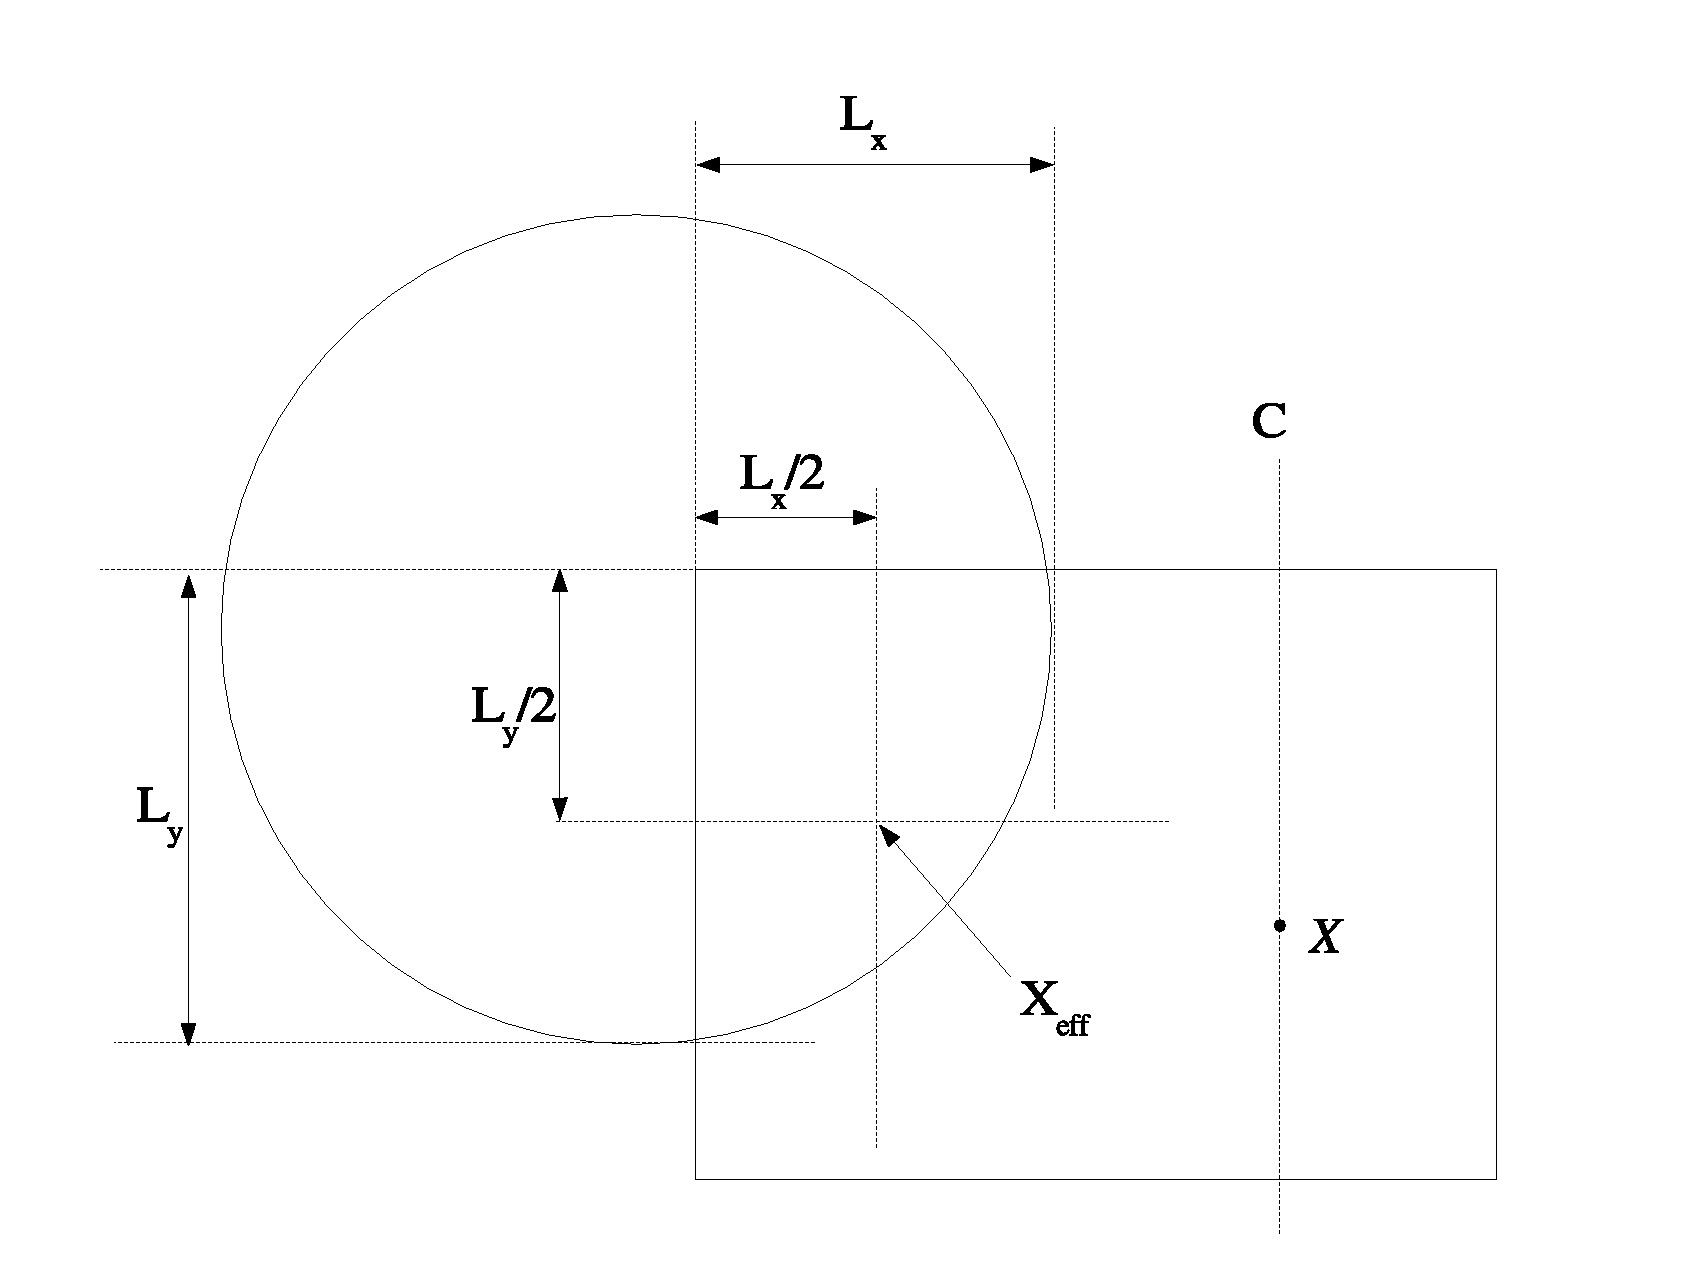
\includegraphics[clip]{CM.eps}}
\caption{ A schematic diagram to explain the Center of Mass (CM)
partitioning scheme.  A sphere of Bragg-Slater~\cite{Slater_64v41}
radius $R_i$ centered on the atom $i$ is drawn for each atom (for
simplicity, only one atom is considered in this case).  The volume of
box-sphere intersection is approximated by $L_x L_y L_z$, where the
$L_x$ is the range of intersection between the sphere and the box in
the $x$ direction. $L_y$ and $L_z$ are calculated in a similar
way. For simplicity we have assumed that the effective charge
$Z_{\mathrm{eff},i}$ is centered at ${\bf X}_{\mathrm{eff}}$. Also
shown is a cutting plane C passing through the center of mass ${\bf
X}$.  }\label{fig:CM}
\end{figure}
% END FIGURE
}

In the Center of Mass (CM) partitioning scheme, we make a plausible
assumption that the computing time for a subbox is proportional to the
total electron charge in the box.  To partition a BBox (see
Figure~\ref{fig:CM}), we first calculate the center of the electron
charge, which we have loosely called the ``center of mass''.  We
assume that the electron charge due to an atom $i$ is smeared out
evenly in a sphere of radius $R_i$, which we have taken to be the
Bragg-Slater radius~\cite{Slater_64v41} for the atom.  The
Bragg-Slater radius for an atom is the empirical atomic radius,
derived from the fact that two atoms forming a bond in a crystal or
molecule gives an approximate value of the internuclear distance. It
is observed that inter-atomic bond lengths in solids and molecules,
whether ionic or covalent, are approximately equal to pairwise sums of
unique atomic radii~\cite{Slater_64v41}.  The center of mass (charge)
${\bf X}$ is given by
\begin{equation}
{\bf X} = \frac{\sum_{i} Z_{\mathrm{eff},i} {\bf X}_{\mathrm{eff},i}}
{\sum_{i} Z_{\mathrm{eff},i}}
\label{eq:X}
\end{equation}
where $Z_{\mathrm{eff},i} = Z_i (L_x L_y L_z/V_i)$, with $V_i = 4\pi
R_i^3/3$.  The symbols $L_x$, $L_y$, $L_z$, and ${\bf
X}_{\mathrm{eff},i}$ are explained in Figure~\ref{fig:CM}. The index
$i$ in Eq.~(\ref{eq:X}) runs through all atoms which overlap (totally
or partially) with the box to be partitioned.  In practice, we only
calculate one component of ${\bf X}$, which is along the largest
dimension of the box, since only one cutting plane is passing through
${\bf X}$.  Each of the two subboxes after a CM partitioning may be
subjected to another CM partitioning.  For simplicity, we always
partition the root BBox in such a way that the number of the subboxes
is a power of two, even though this restriction can be dropped easily.
In a parallel calculation, only one processor will perform the serial
CM partition and broadcast the dimensions of subboxes to all other
processors. It is important to emphasize that although the CM
partitioning scheme might not give a good load balance, it does serve
as a cheap and good starting partition for parallel HiCu.  This is not
a problem even for a large system because we can use a reasonably
large local error threshold $\tau$ and a minimal basis set to start a
calculation while the Equal Time partitioning scheme, to be explained
in Subsection~\ref{subsec:Equal Time}, will improve the efficiency in
subsequent SCF cycles.  One can then switch to a better basis set or
lower the threshold $\tau$ during the iterative calculations.

\subsection{Equal Time partitioning scheme}
\label{subsec:Equal Time}
\commentoutA{
% BEGIN FIGURE
\begin{figure}[t]
\resizebox*{3.5in}{!}{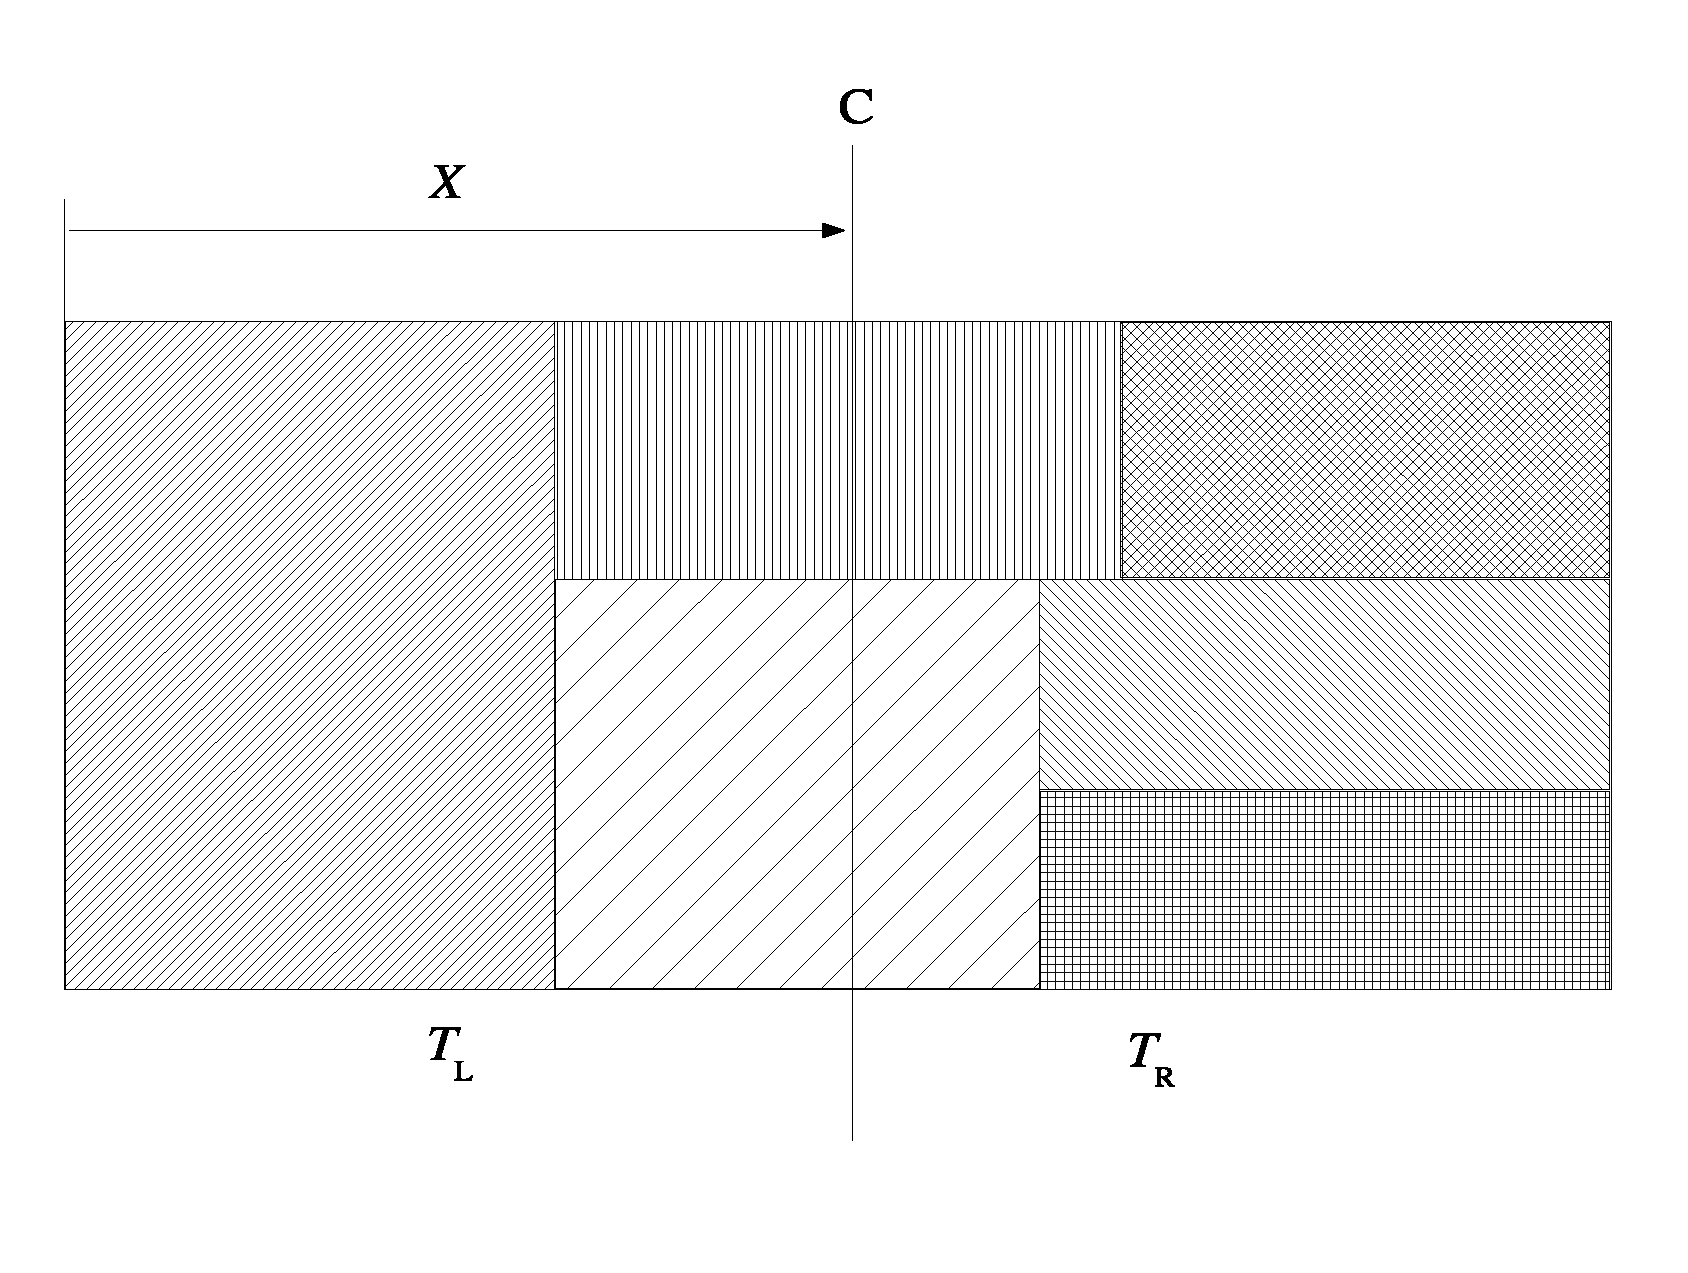
\includegraphics[clip]{ET.eps}}
\caption{A schematic diagram to illustrate the Equal Time (ET) partitioning
scheme.  For simplicity a two-dimensional analog is used. The
rectangles represent the bounding ``boxes'' of the leaf nodes in a
CubeTree.  Different shades are used for different rectangles to
indicate that the leaf-node times are different in general. The
distance of the cutting line C from the left edge, $x$, is determined
by the condition that the sum of the leaf-node times on both sides of
the partition line is equal (i.e., $T_L = T_R$).  Notice that we have
chosen the direction for partitioning as the direction which gives the
largest dimension.}
\label{fig:shiftline}
\end{figure}
% END FIGURE
}

Next we discuss measurement approaches to domain decomposition, with
the goal of repartitioning the root BBox based on workload information
collected during CubeTree construction in the previous SCF cycle.  
By analogy with other parallel methods for computation of $\Kxc$,
we first considered distributing an equal share of grid points, naively 
reasoning that work load would be proportional to their number. 
If we evaluated the density using conventional methods, this would 
certainly be so.  However, this is not a reliable tack because 
each leaf node interacts with the RhoTree in a different way, always attempting to 
minimize the total work load.  Also, because each interaction of a leaf 
node with the RhoTree is so non-uniform, the simple 
interaction counting mechanisms employed by parallel $N$-Body methods~\cite{JPilkington96,warren:92_article,Grama94_article,Warren95b,Singh93,Singh_95v27,Grama_98v24}
are not a viable alternative.  This line of reasoning led us in the
development of Equal Time (ET) partitioning,  which uses the elapsed
wall time associated with Cartesian sub-volumes (here the leaf nodes)
to predict a good load balance in the next iteration.

In the ET partitioning of HiCu, the leaf-node time is stored along with other
attributes in a variable of type CubeNode~\cite{MChallacombe00A}.
With all processors holding leaf-node times in their respective local
CubeTrees, ET creates a new domain decomposition by recursively
partitioning a box into two subboxes such that each subbox carries
approximately the same total leaf-node time (hence ``Equal Time'').
At the end of the decomposition we are left with $\Np$ ET BBoxes in
which to construct a HiCu grid.  The astute reader will by now realize
this construction requires $\Np$ to be a power of two, and that errors
made early in the decomposition will propagate to the lowest level.
These are simple conveniences, which can be easily addressed in future
should they prove problematic.  We have used a robust bisection
method~\cite{WPress92} to find the plane which equally (to some
threshold) divides the workload in half (see Figure
\ref{fig:shiftline}). Notice that the cutting direction may be varied
at each level of the recursion to avoid elongated ET BBoxes which
could lead to poorly-balanced workloads. Our decomposition always
choses a direction which cuts along the largest box dimension, since
the cubature rules will work best for leaf nodes close to cubic~\cite{Stroud71}.

The application of ET to HiCu centers around interaction of the 
CubeTree leaf nodes with the RhoTree.  This implementation does not account
for the time taken to build each matrix element by traversing the CubeTree.
This is because of the close homology between basis function products
and the electron density; they visit nearly identical portions of the
CubeTree.  However, if this homology did not exist, ET  could
associate primitive basis function products with Cartesian sub-volumes 
and wall times, using the combined information to load balance.

A working hypothesis of ET partitioning applied to HiCU is that the sum of 
leaf-node times for the root BBox is constant irrespective of sectioning.  In
practice this assumption is only approximately true, as the total number of leaf nodes and
their times may fluctuate if the cutting planes are shifted. This is 
because with each new partitioning the CubeTree will
readjust, potentially using a different number of leaf nodes to satisfy
$\delta<\tau$.  Also, as the time to create each leaf node depends on
its size and position, readjustments will lead to leaf-node times that
are somewhat different. Finally, variation of the density and hence
the grid will occur in all but the last few SCF cycles.  All of these
factors work against ET partitioning.  The magnitude of these factors
depends on the granularity of the partition, as will be seen in 
Section~\ref{sec:results}.


\commentoutA{
\begin{figure}[t]
\resizebox*{3.5in}{!}{\includegraphics[clip]{taxol.eps}}
\caption{The taxol electron density color-mapped with the electrostatic potential.}
\end{figure}
}

\section{Data parallel approach}
\label{sec:data-locality}

Data parallelism is essential for scalable algorithms, as data
replication stands to exhaust local memory and throttle communications
with increasing $N$ and $\Np$.  For parallel HiCu, each of the ET
BBoxes requires only local information about the electron density.  By
building a {\it locally essential RhoTree}, which is {\it just}
sufficient to create the grid in an ET BBox, redundant replication of
data is avoided.  Another advantage is that the smaller locally essential 
RhoTree is more efficient to traverse relative to the entire RhoTree
that would be encountered in a replicated data scheme. This reduced complexity 
due to data parallelism can lead to superlinear speedups as shown in 
Section\ref{sec:results}.

Data parallelism begins with a distributed atom-blocked compressed
sparse row (DBCSR)~\cite{MChallacombe00B} density matrix ${\bf
P}^{p}$, which is used by program {\sc MakeRho} to create an
intermediate distributed Hermite-Gaussian
(HG)~\cite{Ahmadi95,MChallacombe97,MChallacombe00A} density $\rho^p$.
The intermediate density consists of primitive distributions
associated with only the rows spanned by ${\bf P}^p$.  {\sc MakeRho}
writes $\rho^p$ to local disk in parallel, avoiding IO and network
bottlenecks.  As an aside, this is the same density also used by
program {\sc
QCTC}~\cite{MChallacombe96,MChallacombe96B,MChallacombe97}.  The
intermediate density $\rho^p$ is generally insufficient to build a
CubeTree in an ET BBox.  Communication involving all processors now
occurs to construct the locally essential density $\rho^p_{\rm LE}$.  
Ultimately, sophisticated ordering and scheduling techniques
could be used to reduce complexity of this step.  So far however, we
have found no degradation of performance due to this redistribution.
Construction of $\rho^p_{\rm LE}$ involves all processes going
through their local primitive density distributions, performing
box-box overlap tests as described in
Ref.~\onlinecite{MChallacombe00A} to determine the exchange of data.
After this redistribution of densities, construction of the locally
essential RhoTree, local CubeTree, and local partially summed
exchange-correlation matrix (denoted by ${\bf L}_{\mathrm{xc}}^{p}$)
proceeds independently.  The local, partially summed
exchange-correlation matrix results from numerical integration of all
primitive basis function products in the ET BBox, and is related to the full
exchange-correlation matrix $\Kxc$ by
\begin{equation}
\Kxc = \sum_{p=1}^{\Np}{\bf L}_{\mathrm{xc}}^{p}~,
\label{eq:kxcp}
\end{equation}
although the summation in Eq.~(\ref{eq:kxcp}) is not explicitly
carried out.  Rather, ${\bf L}_{\mathrm{xc}}^{p}$ is redistributed and
resumed to yield a non-overlapping row-distributed ${\bf
K}_{\mathrm{xc}}^{p}$.

\commentoutA{
\begin{figure}[t]
\resizebox*{3.5in}{!}{\includegraphics[clip]{taxol_speedup.eps}}
\caption{Scaling of parallel HiCu on taxol (C$_{47}$H$_{51}$NO$_{14}$)
RPBE/3-21G, with $\tau = 1.0 \times 10^{-6}$. Speedups are relative to
a 2-processor calculation.}\label{fig:taxol}
\end{figure}
}

As $\Np$ becomes large, the ET BBox will become small and the
corresponding local exchange-correlation matrix will become very
sparse.  During matrix construction there can be significant overheads
associated with simple box-box testing of primitive basis function
product BBox overlaps with the ET BBox.  This problem is also
encountered for periodic HiCu~\cite{CTymczak03}, where a double sum
over lattice vectors leads to a substantial fraction of basis function
products that are outside the root BBox.  Our solution, described in
detail elsewhere~\cite{MChallacombe03A}, is to perform a high level test between
basis function products in an atom-atom pair and the ET BBox using a
cylinder-box overlap test.


Another potential complexity encountered with fine grained parallelism
involves the redistribution and resummation of ${\bf
L}_{\mathrm{xc}}^{p}$.  If one uses sparse-matrix data structures
related to the standard CSR~\cite{FGustavson78,SPissanetzky84} data
structure such as the DBCSR or BCSR constructs~\cite{MChallacombe00B},
the resummation of very many small sparse matrices can lead to large
copy overheads.  We have developed the Fast Matrix~\cite{MChallacombe03B} 
(FastMat) data structure to address this problem, in which all rows are 
connected by a linear linked list, while each row is represented by a binary tree.
This new construct has a low overhead for random insertions and
updates of atom-atom blocks.  It also allows many operations such as
matrix-matrix addition and matrix truncation to be done in-place,
reducing both memory and copy overheads.

\section{Implementation}
\label{sec:implementation}
\commentoutA{
\begin{figure}[t]
\resizebox*{3.5in}{!}{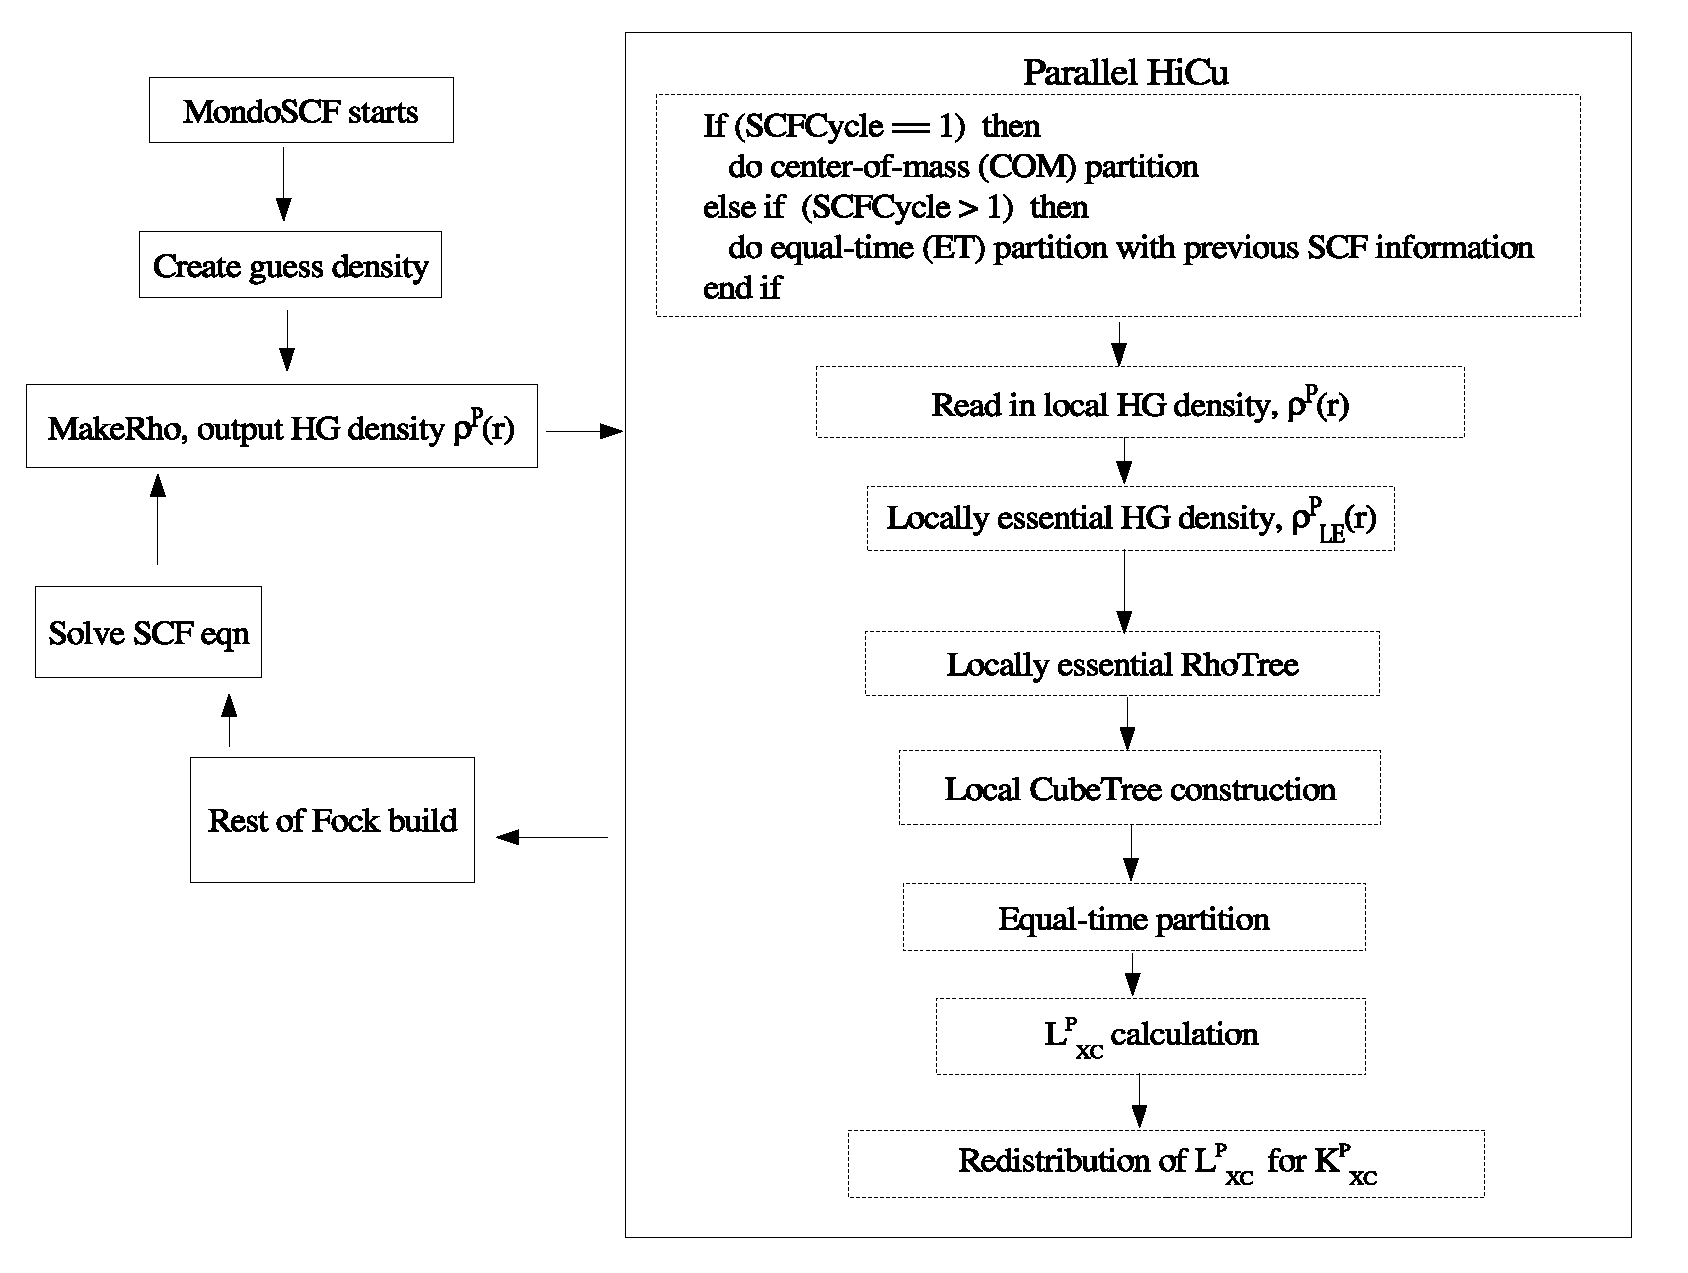
\includegraphics[clip]{PHiCuFlow.eps}}
\caption{The general flow of {\sc MondoSCF}, with parallel HiCu subroutine
expanded.  Refer to Section~\ref{sec:implementation} for more
details.}
\label{fig:parahicu}
\end{figure}
}

We have implemented the parallel HiCu algorithm in {\sc
MondoSCF}~\cite{Mondo}, a suite of programs for linear scaling
electronic structure theory and {\it ab initio}\/ molecular dynamics.
Figure~\ref{fig:parahicu} shows the general flow of an SCF cycle, with
expanded detail of parallel HiCu.  {\sc MondoSCF} has been written in
Fortran 90/95 with the message-passing library MPI~\cite{mpi}.
Leaf-node times are calculated with the {\tt MPI\_WTIME} MPI function.

\section{Results}
\label{sec:results}

\commentoutA{
\begin{figure}[t]
\resizebox*{3.5in}{!}{\includegraphics[clip]{3-21G_good_div10.eps}}
\caption{Scaling of parallel HiCu on (H$_2$O)$_{110}$ RPBE/3-21G, with
$\tau = 1.0 \times 10^{-6}$. Speedups are relative to a 2-processor
calculation.}\label{fig:waterscaling}
\end{figure}
}

We have performed scaling tests on taxol and a cluster of 110 water
molecules with $2^n$ processors, where $n$ typically ranges from 1 to
7.  These systems are chosen because they are highly inhomogeneous,
three-dimensional system posing a challenge to parallel HiCu.  
All runs are performed on a single SGI Origin 2000
with 128 (250 MHz MIPS R10000 MIPS) processors.

We start the calculations with the STO-3G basis set and a large 
threshold $\tau$, switch to the 3-21G basis set using our mixed
integral approach, and run for three SCF cycles.  The density matrix
${\bf P}$ is saved to disk and scaling tests of parallel HiCu are
performed.  Timings for parallel HiCu are taken at the fourth cycle where the
Center of Mass partition is used, and at the fifth cycle where the
Equal Time partition is used. The procedure of switching the basis set and 
iterating for a few SCF cycles places the electron density in the middle 
of convergence.  This is not really necessary, as performance is pretty 
insensitive to SCF cycle.  


The result of taxol scaling tests is shown in Figure~\ref{fig:taxol},
where the Center of Mass partitions perform rather poorly past 16 processors, with
a speedup of only 22.4 obtained at 64 processors.  However, the Equal
Time partitions give good scaling results compared to the ideal
speedup, obtaining a speedup of 60.8 with 64 processors.  We note that
our result of a speedup of 7.03 with 8 processors compares favorably
with the speedup of about 6.0 of Sosa {\it et al.}~\cite{Sosa_00v26},
which is for an entire single-point energy calculation.

Similar scaling tests have been performed on a cluster of 110 water
molecules.  Figure~\ref{fig:waterscaling} shows that the Center of
Mass partition gives a better speedup than in the case of taxol.
Equal Time repartitioning is highly effective.  The speedup
is almost ideal up to 64 processors. We observe a superlinear speedup
at 32 processors, which is a medium-grained calculation.  We attribute
the superlinear speedup to a good load balance and to reduced
complexity associated with data parallelism, where the memory access
time has been greatly reduced with a smaller RhoTree.  The speedup
with 128 processors degrades slightly to 112.64 (an efficiency of
88\%).  Still, this is an encouraging result as the 128-processor run
corresponds to very fine-grained parallelism, with less than one heavy
atom per processor. The reason for this degraded efficiency is not due
to communication overhead but to intrinsic limitations in the ET
scheme associated with fluctuations in the leaf-node count and small
non-conservation of total times as explained in
\ref{subsec:Equal Time}.  While there are almost certainly ways to
overcome/compensate for these effects, we feel that the overall
performance of ET for parallel HiCu is outstanding.  To explore
the behavior of the current implementation with $\Np \sim 1024 $ will 
require a fully parallel {\sc MondoSCF}, which we are actively pursuing.

\section{Conclusions}
\label{sec:conclusions}

We have developed an efficient and general load balancing technique,
Equal Time (ET) partitioning, and used it in data parallel
implementation of the linear scaling Hierarchical Cubature (HiCu)
algorithm for numerical integration of the exchange-correlation
matrix.  In the ET approach, strong spatial irregularities in the work
load are overcome by exploiting temporal locality between iterations.
We expect ET to also exploit this effect between geometry steps in an
optimization or molecular dynamics run.  In this data parallel
implementation, quantum locality has been used to reduce
communications between processors, to lower memory usage and to reduce
the computational complexity associated with traversal of the RhoTree.
In some cases, this last effect can lead to superlinear speedups for
medium grained calculations.

To the best of our knowledge, Equal Time partitioning is the first
measurement based load balancing strategy applied to Quantum
Chemistry.  While ET partitioning shares some commonalities with
partitioning schemes for parallel $N$-body tree-code solvers such as
Orthogonal Recursive Bisection (ORB)~\cite{warren:92_article} and
Costzones~\cite{Singh93}, ET differs by (i) using exact load timing
information rather than counting the number of interactions as in the
ORB and Costzones methods and (ii) associating this load with
rectilinear partitioning of Cartesian space rather than particle
groupings (ORB) or nodes in a tree (Costzones).  These are important
distinctions for Quantum Chemistry.  Often methods are much more
complicated than the simple $N$-body problem.  Measured loads
encompass irregularities associated with different Gaussian extents,
non-uniform access patterns, etc.~that cannot be accounted for by
counting interactions.  Also, because we are often doing several
complicated things at once, attaching work loads to a portion of
3D space is a convenient catch-all that can be associated with most
objects and processes: basis function products and matrix construction,
electron densities and grid construction, etc.  

Our parallel approach to construction of $\Kxc$ differs fundamentally
from other all-electron approaches in that (i) we do not employ Becke
weights and (ii) we employ measurement based load balancing.  It is
also different from many implementations in that (iii) it is data
parallel.  In addition to the numerical issues discussed in Section
\ref{sec:intro}, we believe the non-overlapping Cartesian subdivision
used by HiCu enables a more straight forward approach to data locality
and domain decomposition.  Both the replicated data and the
master-slave approach have well known shortcomings for fine grained
massive parallelism, which have been avoided here.  With less than one
heavy atom per processor, data parallel HiCu using ET partitioning is
88\% efficient with 128 processors.  The predominent cause of
deviation from the ideal is due to basic non-linearities in ET
partitioning of the HiCu grid, rather than overheads associated with
inefficient data structures or communication.

\begin{acknowledgments}
This work has been carried out under the auspices of the US Department
of Energy under contract W-7405-ENG-36 and the ASCI project.  The
Advanced Computing Laboratory of Los Alamos National Laboratory, Los
Alamos, NM 87545 is acknowledged.  This work was performed on
computing resources located at this facility.
\end{acknowledgments}


\bibliographystyle{apsrmp} \bibliography{mondo}

\pagebreak

\commentoutB{

\pagebreak

\begin{center}
\bf  FIGURES
\end{center}

\begin{figure}[h]
\caption{ A schematic diagram to explain the Center of Mass (CM)
partitioning scheme.  A sphere of Bragg-Slater~\cite{Slater_64v41}
radius $R_i$ centered on the atom $i$ is drawn for each atom (for
simplicity, only one atom is considered in this case).  The volume of
box-sphere intersection is approximated by $L_x L_y L_z$, where the
$L_x$ is the range of intersection between the sphere and the box in
the $x$ direction. $L_y$ and $L_z$ are calculated in a similar
way. For simplicity we have assumed that the effective charge
$Z_{\mathrm{eff},i}$ is centered at ${\bf X}_{\mathrm{eff}}$. Also
shown is a cutting plane C passing through the center of mass ${\bf
X}$.  }\label{fig:CM}
\end{figure}

\begin{figure}[h]
\caption{A schematic diagram to illustrate the Equal Time (ET) partitioning
scheme.  For simplicity a two-dimensional analog is used. The
rectangles represent the bounding ``boxes'' of the leaf nodes in a
CubeTree.  Different shades are used for different rectangles to
indicate that the leaf-node times are different in general. The
distance of the cutting line C from the left edge, $x$, is determined
by the condition that the sum of the leaf-node times on both sides of
the partition line C is equal (i.e., $T_L = T_R$).  Notice that we
have chosen the direction for partitioning as the direction which
gives the largest dimension.}
\label{fig:shiftline}
\end{figure}

\begin{figure}[h]
\caption{The general flow of {\sc MondoSCF}, with parallel HiCu subroutine
expanded.  Refer to the text for more details.}
\label{fig:parahicu}
\end{figure}
 
\begin{figure}[h]
\caption{Scaling of parallel HiCu on taxol (C$_{47}$H$_{51}$NO$_{14}$)
RPBE/3-21G, with $\tau = 1.0 \times 10^{-6}$. Speedups are relative to
a 2-processor calculation.}\label{fig:taxol}
\end{figure}

\begin{figure}[h]
\caption{Scaling of parallel HiCu on (H$_2$O)$_{110}$ RPBE/3-21G, with
$\tau = 1.0 \times 10^{-6}$. Speedups are relative to a 2-processor
calculation.}\label{fig:waterscaling}
\end{figure}

\begin{figure}[h]
\caption{An illustrative example to show the general Equal Time partitioning scheme, for the case of $m=5$.}\label{fig:binary}
\end{figure}

%\clearpage
\pagebreak

\begin{center}
Figure 1, C.~K.~Gan and M.~Challacombe \\[1.cm]
\resizebox*{6.0in}{!}{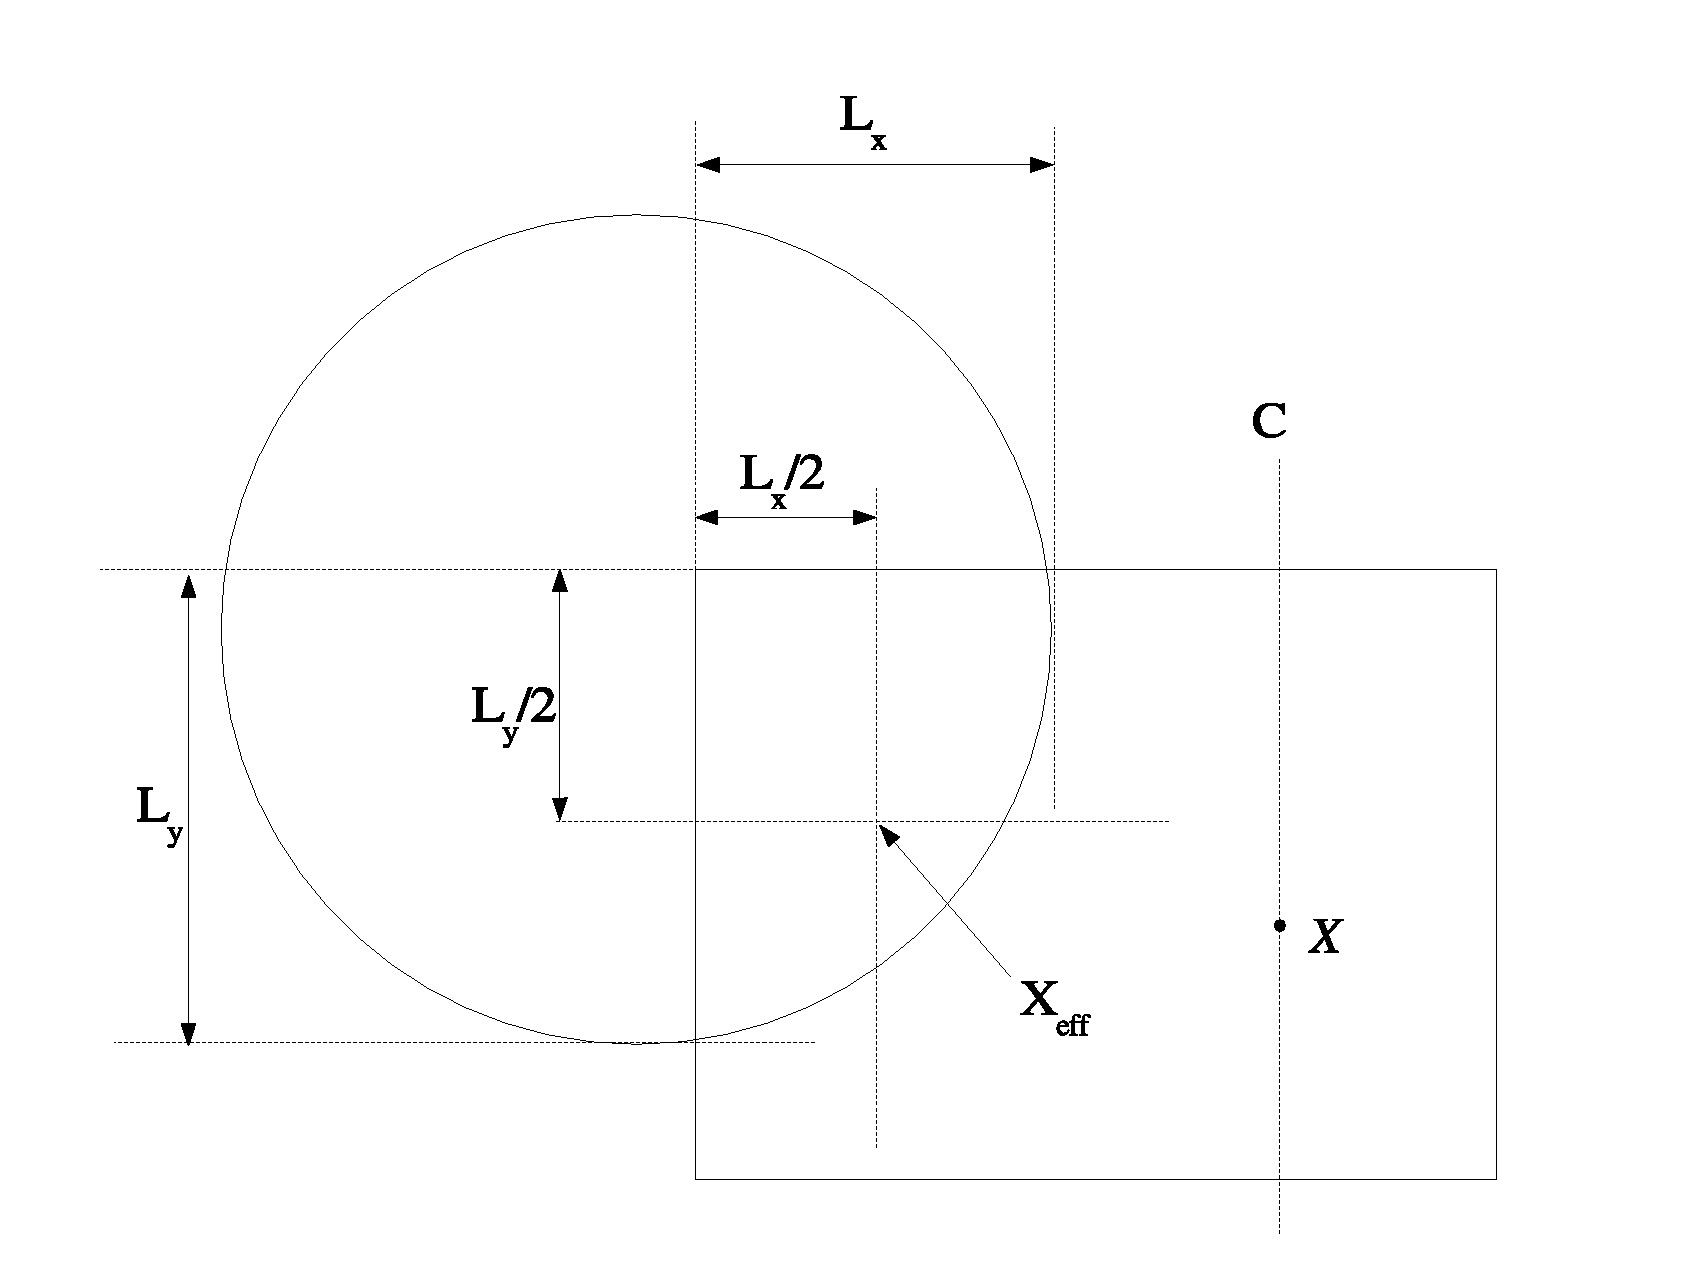
\includegraphics[clip]{CM.eps}}
\end{center}

\pagebreak
\begin{center}
Figure 2, C.~K.~Gan and M.~Challacombe \\[1.cm]
\resizebox*{6.0in}{!}{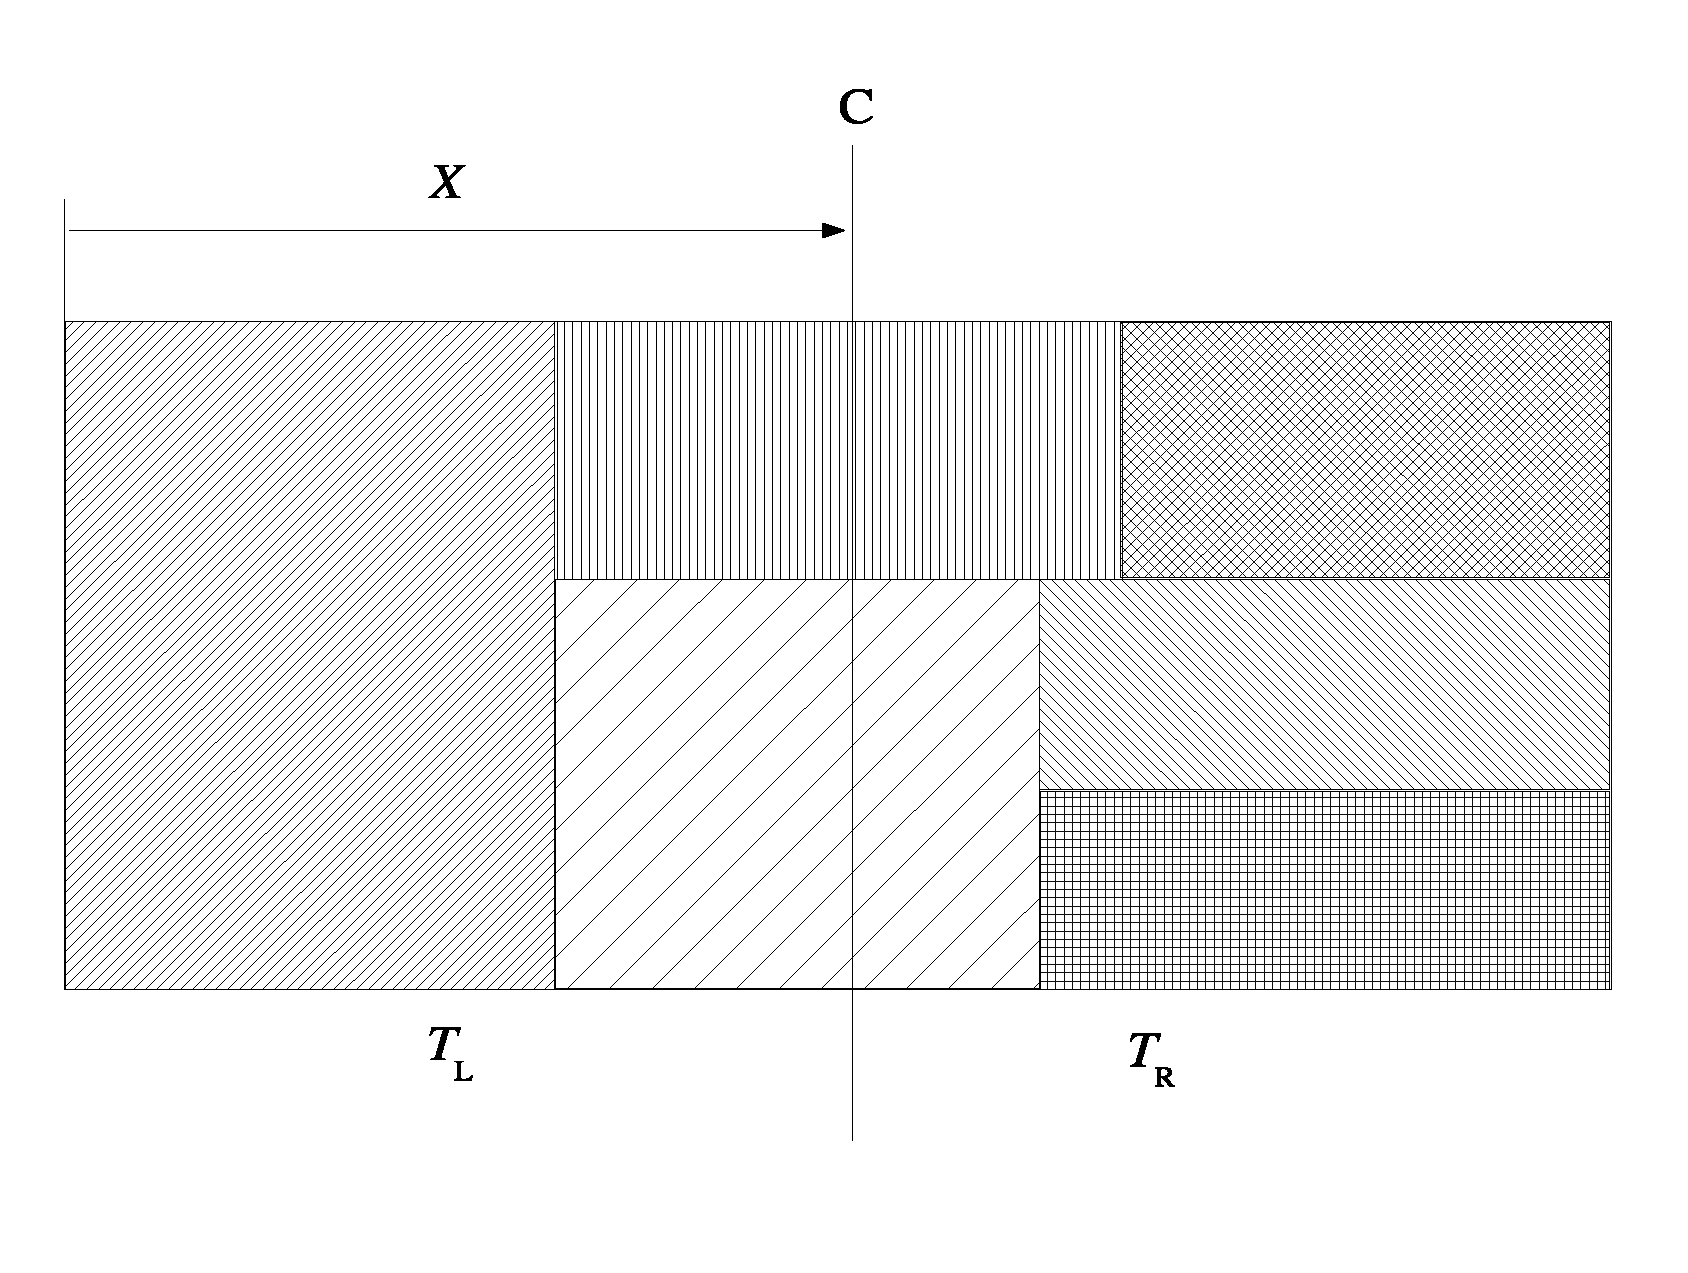
\includegraphics[clip]{ET.eps}}
\end{center}

\pagebreak
\begin{center}
Figure 3, C.~K.~Gan and M.~Challacombe \\[1.cm]
\resizebox*{6.0in}{!}{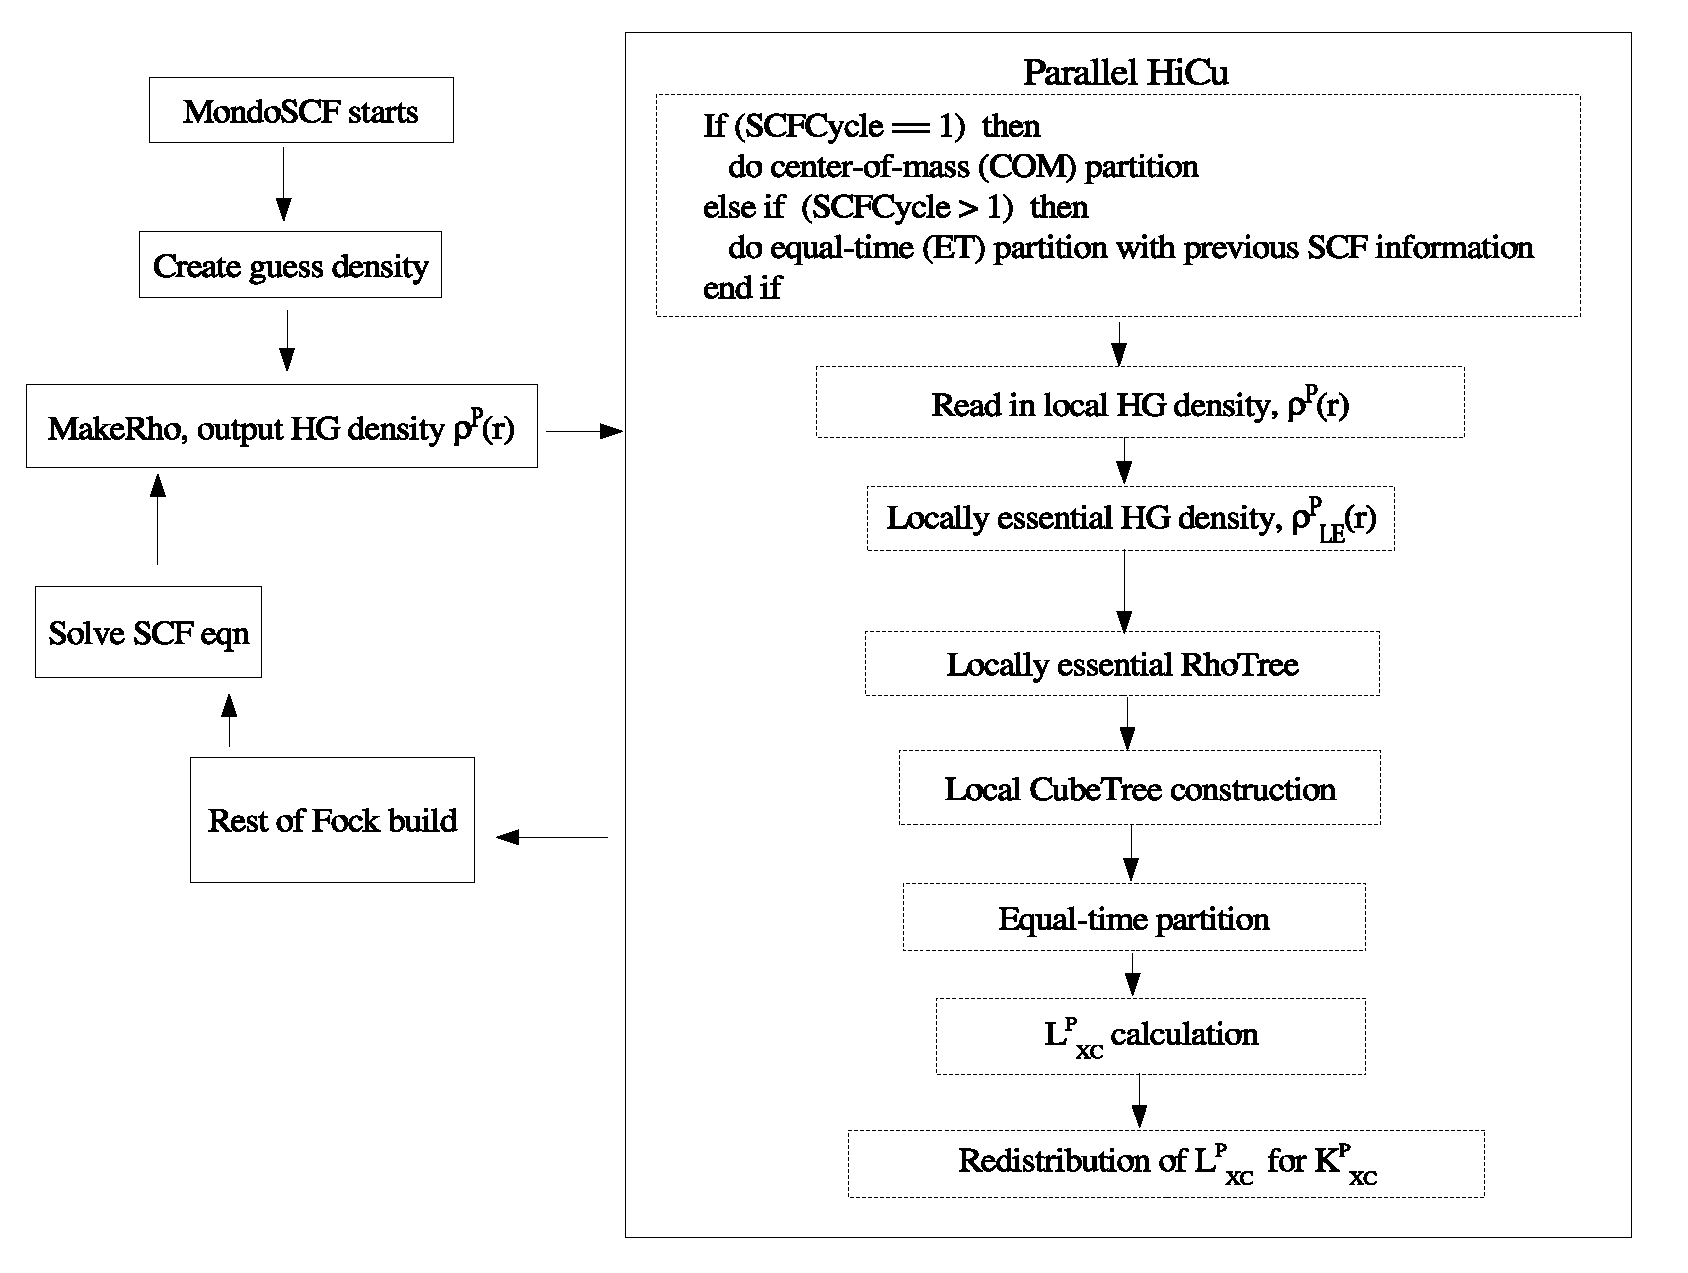
\includegraphics[clip]{PHiCuFlow.eps}}
\end{center}

\pagebreak
\begin{center}
Figure 4, C.~K.~Gan and M.~Challacombe \\[1.cm]
\resizebox*{6.0in}{!}{\includegraphics[clip]{taxol_speedup.eps}}
\end{center}

\pagebreak
\begin{center}
Figure 5, C.~K.~Gan and M.~Challacombe \\[1.cm]
\resizebox*{6.0in}{!}{\includegraphics[clip]{3-21G_good_div10.eps}}
\end{center}

\pagebreak
\begin{center}
Figure x, C.~K.~Gan and M.~Challacombe \\[1.cm]
\resizebox*{6.0in}{!}{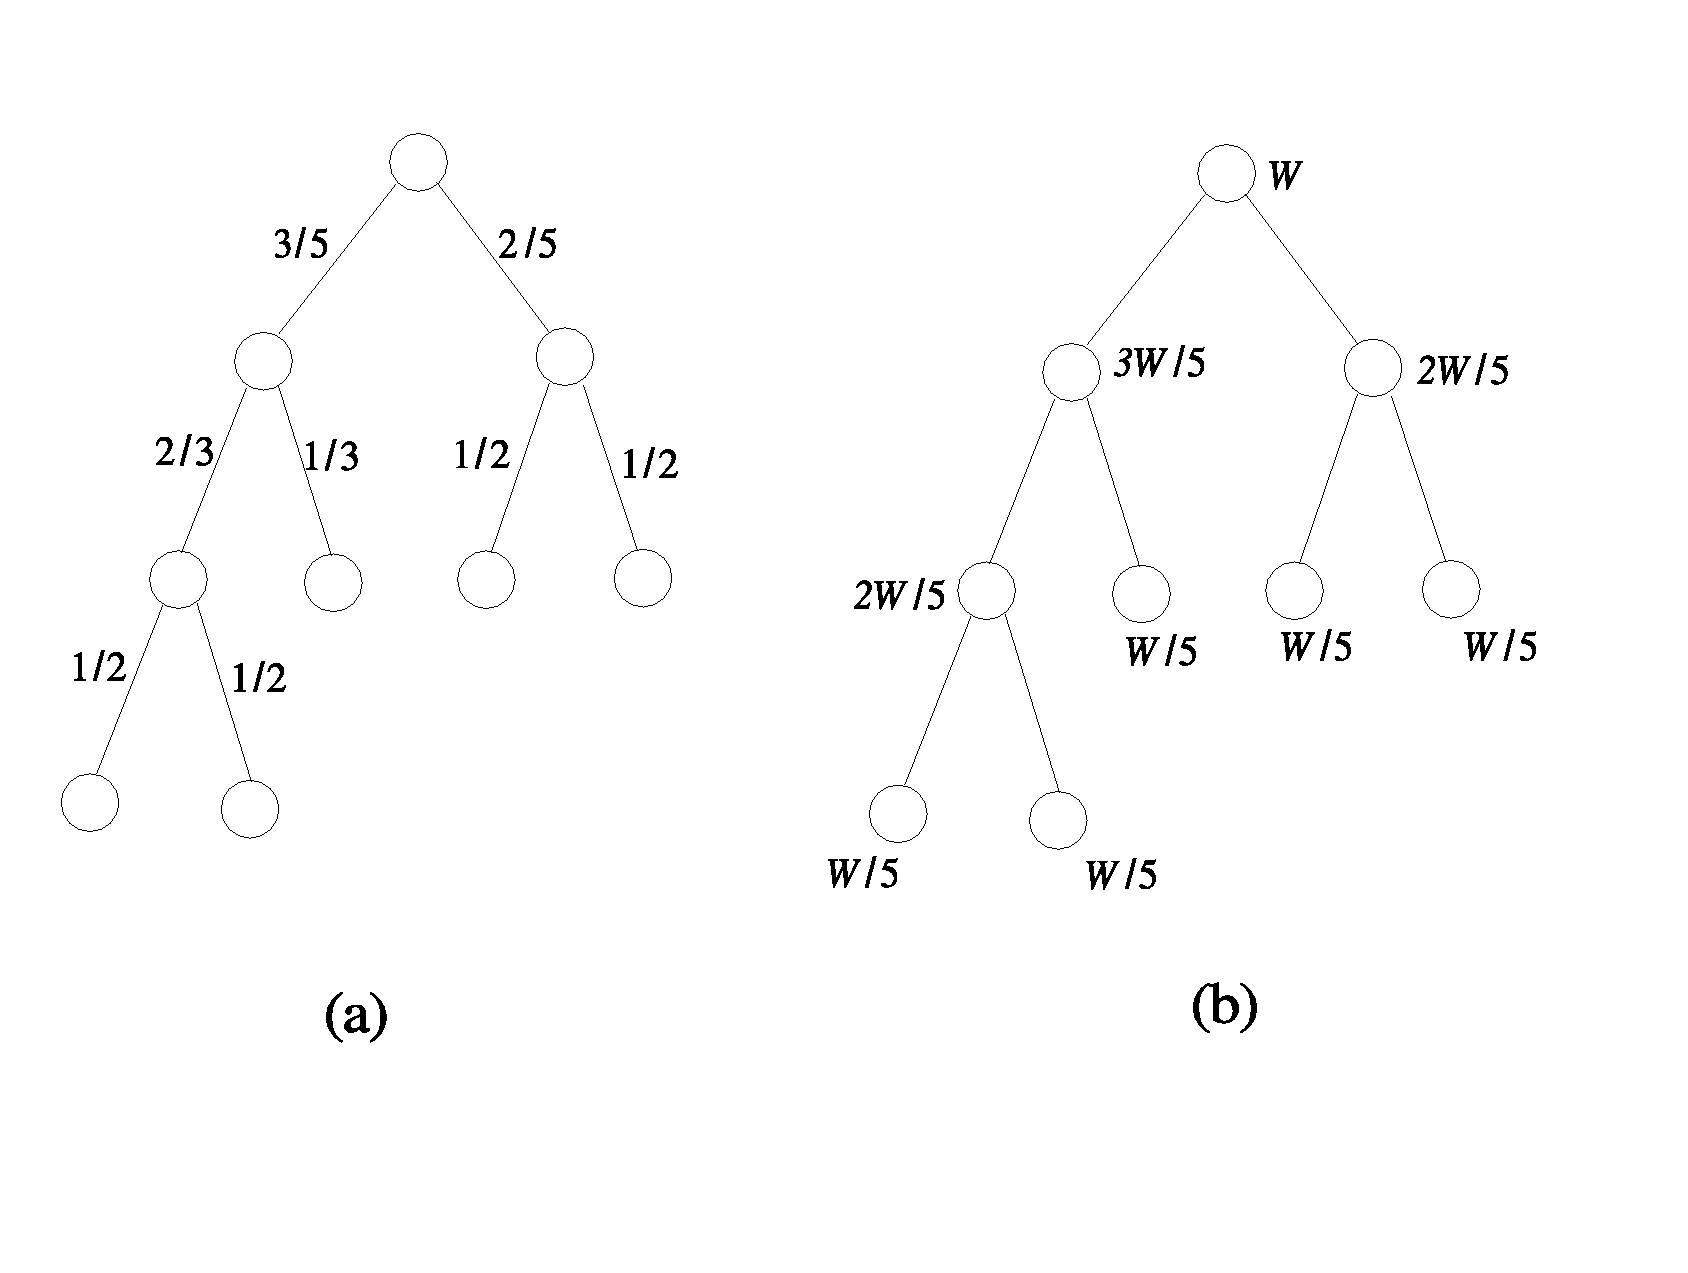
\includegraphics[clip]{binary.eps}}
\end{center}
}

\appendix
\section{A general Equal Time partitioning scheme}
\label{appex:GET}
In this appendix we describe a general Equal Time partitioning scheme where 
the number of subboxes, denoted by $m$, is not restricted to a power of two.
To facilitate this general 
partitioning, we first create a binary tree with $m$ leaf nodes, with
the condition that the depths between any two leaf nodes do not differ by more
than one. 
Next we associate the edges connecting a parent node to its left and 
right child nodes with edge weights equal to 
$n_{\scriptscriptstyle\mathrm{L}}/(n_{\scriptscriptstyle\mathrm{L}}+n_{\scriptscriptstyle\mathrm{R}})$
and $n_{\scriptscriptstyle\mathrm{R}}/(n_{\scriptscriptstyle\mathrm{L}}+n_{\scriptscriptstyle\mathrm{R}})$, respectively. 
Here $n_{\scriptscriptstyle\mathrm{L}}$ ($n_{\scriptscriptstyle\mathrm{R}}$)
is the number of left (right) leaf nodes of the parent node. 
Fig.~\ref{fig:binary}(a) shows a binary tree and all the edge weights 
for the case of $m=5$.
With these edge weights, it is a fairly simple matter 
to partition a total workload $W$ into $m$ equal workloads. Starting
from the root node,
we divide the workload in a parent node
according to the ratio of the edge weights, i.e. $n_{\scriptscriptstyle\mathrm{L}} : n_{\scriptscriptstyle\mathrm{R}} $. Using this procedure, all
leaf nodes will have a workload of $W/m$. Fig.~\ref{fig:binary}(b) shows the 
detailed workload information in all nodes for the case of $m=5$. In a domain
decomposition of a root BBox, a bisection search can be used to partition
a box into 2 subboxes with a workload ratio equals to 
$n_{\scriptscriptstyle\mathrm{L}} : n_{\scriptscriptstyle\mathrm{R}}$,
which can be easily read off from the edge weights of the binary tree.
It turns out that ``power-of-two'' Equal Time partitioning scheme 
explained in section~\ref{subsec:Equal Time} is a special 
case of this general partitioning scheme. 
\end{document}
